% This is samplepaper.tex, a sample chapter demonstrating the
% LLNCS macro package for Springer Computer Science proceedings;
% Version 2.20 of 2017/10/04
%
\documentclass[runningheads]{llncs}
%
\usepackage{graphicx}
\usepackage{float}
%% Save the class definition of \subparagraph
\let\llncssubparagraph\subparagraph
%% Provide a definition to \subparagraph to keep titlesec happy
\let\subparagraph\paragraph
%% Load titlesec
\usepackage[compact]{titlesec}
%% Revert \subparagraph to the llncs definition
\let\subparagraph\llncssubparagraph
% Used for displaying a sample figure. If possible, figure files should
% be included in EPS format.
%
% If you use the hyperref package, please uncomment the following line
% to display URLs in blue roman font according to Springer's eBook style:
% \renewcommand\UrlFont{\color{blue}\rmfamily}
\titlespacing{\subsubsection}{0pt}{0.5\baselineskip}{0.5\baselineskip}
\begin{document}
%
\title{Heuristic Search Practice. TSP with A*, SPA* and GA\thanks{Supported by University of Oviedo}}
%
%\titlerunning{Abbreviated paper title}
% If the paper title is too long for the running head, you can set
% an abbreviated paper title here
%
\author{Israel Solís Iglesias\orcidID{UO282162} \and
Omar Teixeira González\orcidID{UO281847} \and
David Leszek Warzynski Abril\orcidID{UO278968}\thanks{The authors have been arranged in alphabetical order based on their surnames}}
%
\authorrunning{Solís, I and Teixeira, O. and Warzynski, D.L.}
% First names are abbreviated in the running head.
% If there are more than two authors, 'et al.' is used.
%
\institute{Inteligent Systems, School of Computer Engineering, University of Oviedo, Oviedo, Spain\\
\email{\{UO282162,UO281847,UO278968\}@uniovi.es}\\
\url{https://ingenieriainformatica.uniovi.es/}}
%
\maketitle              % typeset the header of the contribution
%

\begin{abstract}
The Traveling Salesman Problem (TSP) poses the challenge of a traveler commencing from a city and navigating through all available cities exactly once, ultimately returning to the initial departure city, all while endeavoring to identify the most cost-efficient route. In this article, we will conduct an experimental investigation into solving the TSP utilizing the A* search algorithm and SPA*. These algorithms will be implemented with various heuristics to explore state spaces effectively. Lastly, we will present and compare the results obtained from employing these distinct methods.
    \keywords{A* \and SPA* \and GA \and State space search \and Heuristic \and TSP.}
\end{abstract}

% 
% First paragraph is a general description of the paper and the work that has been done, while the last paragraph is a description of the following content of the paper.
% 
\section{Introduction}
Search algorithms are the foundation of every intelligent system, categorized into two distinct types: uninformed/blind and informed algorithms. This paper delves into informed algorithms, explicitly focusing on A* and SPA*, employing various heuristics and their application to the Traveling Salesman Problem (TSP). A subsequent comparison between these algorithms will be conducted, alongside an exploration of applying genetic algorithms, providing a comprehensive analysis. 

This paper will present comparative analyses through carefully executed experiments, showcasing outcomes in dedicated sections. 

The structure of this article unfolds as follows. Section 2 initiates with an elucidation of the traveling salesman problem. Sections 3, 4, and 5 sequentially expound on search algorithms, their application to the TSP, and the findings of the experimental study. Finally, Section 6 encapsulates the conclusions drawn from this research.

% Explanation of the traveling salesman problem.
% Problem statement, some applications, classical methods of resolution, ...
%
\section{Traveling Salesman Problem (TSP)}
The Traveling Salesman Problem (TSP) is an algorithmic challenge that involves determining the most efficient route, to visit each city exactly once and return to the starting city. The problem dates back to the 18th century, with notable early contributors including Sir William Rowam Hamilton and Thomas Penyngton. However, it wasn't until the 1930s, that Karl Menger delved into the TSP's general form as it is studied today\cite{waterloo-web}.

Over the years, extensive research has revealed a myriad of applications for the TSP, ranging from the drilling of printed circuit boards to computer wiring and vehicle routing.

The TSP can be tackled using both uninformed algorithms, such as Depth-First, and informed algorithms like A* and SPA*. Additionally, genetic algorithms offer another avenue for solving the problem, as elaborated in the subsequent sections\cite{tsp-ta}.

% 
% A description of the algorithms and their most interesting properties, with some citations to the most important books to the most important books and/or articles. It is not necessary to put the pseudo-code of the algorithm, but if it is included, it should be explained in the text.
%
\section{Search algorithms}
\subsection{A* algorithm}
The A* algorithm is a specialization of the Breadth-First (BF) algorithm which incorporates an evaluation heuristic function denoted as $f(n)=g(n)+h(n)$ with: 

\begin{itemize}
    \item \textbf{$g(n)$}. the cost from the start node to $n$.
    \item \textbf{$h(n)$}. the estimate of the cost from $n$ to the end node.
\end{itemize}

Regarding its properties, A* is a complete algorithm, which means, it guarantees to find a solution when there is one. Both its admissibility and consistency are determined by the heuristic $h(n)$ used.

To ensure its admissibility, $h(n)$ must be optimistic, which is to say that $h(n) < h^*(n)$ $\forall n$, where $h^*(n)$ is the best cost from $n$. On the other hand, its consistency is assured when $h(n) > h(n')$ for any node $n'$, a child of a node $n$. When $h(n)$ is admissible, consistent, or both, A* will always yield the optimal solution. Besides, when it is consistent A* will be optimally efficient compared to other similar algorithms with no all "non-pathological" search problems \cite{optimality-astar}.

\subsection{SPA* algorithm}
Static Ponderation A*\cite{theory-book} is classified among $\epsilon$-admissible algorithms, representing a relaxed variant of the A* algorithm. This adaptation becomes necessary when dealing with large-scale problems, compelling a relaxation of the algorithm's admissibility (while still requiring an admissible heuristic). Essentially, while A* guarantees an optimal solution, it may explore more paths to find it. By relaxing this condition, the algorithm traverses fewer nodes, potentially yielding a solution that is not necessarily optimal.

$\epsilon$-admissible algorithms share the characteristic that the obtained solution will have a maximum cost of $(1 + \epsilon)C*$, where $\epsilon > 0$. In essence, a larger $\epsilon$ results in the expansion of fewer nodes on the path to the solution.

In this paper, the SPA* algorithm used, is defined as $f(n) = g(n) + (1 + \epsilon)h(n)$.

% 
% Description of how A* and SPA* are applied to the problem: search space, heu properties of the heuristics, ...In the case of genetic algorithms, the coding, genetic operators, fitness function, ... In the case of genetic algorithms, the encoding, genetic operators, fitness function... must be explained.
%
\section{Application of algorithms to the TSP}
Both search and genetic algorithms have been utilized to discover the path with the minimum cost that traverses all cities and returns to the initial one. 
\subsection{Search algorithms}
A* and SPA* algorithms\cite{stanford-amit} share the same search space and heuristics. However, there is a unique aspect in the case of SPA*, which will be detailed later in this document.

The algorithm initiates by generating the search space, constructing a graph where each node represents a new addition to the path. Four implemented heuristics determine the path, all designed to identify the path with the minimum cost. These four heuristics are as follows:

\begin{itemize}
    \item \textbf{h1}. Based on calculating the sum of edges connecting the remaining cities to be visited, including the current one.
    \item \textbf{h2}. The sum of the $N-k+1$ least costly edges in the residual graph.
    \item \textbf{h3}. The sum of the $N-k+1$ least costly edges in the residual graph, ensuring that each city in the residual graph has a connecting edge.
    \item \textbf{h\_mst}. Cost of a minimum spanning tree of the residual graph.
\end{itemize}   

Specifically, the h3 heuristic consists of giving a list of edges composing the residual graph sorted by cost, progressively adding the edges of the remaining cities, and removing these cities as they are added. Once all cities are included, if the total length of the stored edges is less than N-k+1, where N is the total number of cities and k is the number of cities visited, then add the remaining edges with the lowest cost from the residual graph, regardless of the cities they connect.

\subsection{Genetic algorithms}
The genetic algorithm is segmented into various components, with the initial part focusing on the encoding scheme. This scheme is founded on permutations of the cities $(1, 2,...,n-1)$. 

Another crucial element is the crossover operator, with two operators implemented in this case: Order crossover and Uniform crossover, the first one copies a substring of symbols from the first parent to the child, maintaining order and position, the rest occupy the remaining positions keeping the order they have in the second parent, while the uniform crossover takes a x number of values from the first parent and then takes the rest in relative order from the other parent.

The final component is the fitness function, which calculates the cost of the path from the initial city to itself, navigating through the remaining cities in the order specified by the individual.

% 
% Algorithm results. The results should be shown in tables or figures. Tables and figures should be numbered and should have an explanatory text (caption). They should be referenced in the text (Figure 3 shows ....). The use of graphs versus tables will be positively valued. The use of graphs as opposed to tables will be positively valued. In addition, any table or graph should be adequately explained.
%
\section{Experimental study}
\subsection{Experimental study design}
In the experimentation of this article, the methods described in the previous sections will be compared. Different instances of the TSP will be solved for this comparison: three of them were provided in the class exercises --gr17, gr21 without four cities and gr21 with all cities--, and the last one --fri26--, obtained from \cite{tsplib95}, which also had the last three cities removed.

In all the experiments, two metrics will be collected for the comparison: the execution time and the cost of the best solution found by the method. The execution time and the best solution found in the case of genetic algorithms are something that can vary with each execution. Therefore, these two metrics have been obtained from 10 different runs, and in the results to be presented, you will find the mean and standard deviation over the 10 runs. In the heuristic algorithms, the number of expanded nodes will also be collected.

Specifically, the SPA* algorithm has been employed with all four aforementioned heuristics and with five different $\epsilon$ values $(0.2, 0.4, 0.6, 0.8, 0.99)$ for each heuristic.

The primary specifications of the computer used for experimentation are as follows:
\begin{itemize}
    \item Processor	AMD Ryzen 5 3600 6-Core Processor, 3600 Mhz, 6 Core(s), 12 Logical Processor(s).
    \item RAM 16.0 GB.
\end{itemize}

Talking genetic algorithms, have been used with different parameters, such as the number of population, which has been set to 100, or the number of generations, which oscillates between the values $(100, 150, 200, 250, 300)$. Being more concrete about implementation, it has also been used elitism, to take the best out of the children, mutation (where it changes 2 values from the child) with 10\% probability, and the possibility of choosing among the 2 aforementioned crossover operators.

\subsection{Experimental results}
\subsubsection{Heuristic comparison} 
The results unequivocally indicate that \textit{h2} emerges as the least effective heuristic in terms of expanded nodes. Conversely, \textit{h\_mst} stands out as the most efficient heuristic regarding expanded nodes. However, this advantage is counterbalanced by the time it takes to reach the solution, which can be longer than that of other heuristics in certain instances, as illustrated in Table \ref{tab:astar-results}.

\begin{table}[H]
\centering
\caption{A* Performance Across Multiple Instances of Varying Sizes and Heuristics.}
\label{tab:astar-results}
\resizebox{\textwidth}{!}{
\begin{tabular}{|c|c|c|c|c|c|}
\hline
Instance & Heuristic & Expanded Nodes & Average (Time) & Standard Deviation (Time) & Length (Cost) \\
\hline
gr17 & h1 & 94216 & 11,0028 & 0,72648496 & 2085 \\
     & h2 & 248137 & 23,78591528 & 1,184029394 & \\
     & h3 & 83744 & 13,20123687 & 1,505892807 & \\
     & h\_mst & 30413 & 57,72750638 & 2,823759739 & \\
\hline
gr21-4 & h1 & 3771 & 0,718152571 & 0,540446349 & 2369 \\
      & h2 & 25510 & 23,78591528 & 1,184029394 & \\
      & h3 & 3108 & 1,019539356 & 0,591314004 & \\
      & h\_mst & 269 & 1,551998925 & 0,00507672 & \\
\hline
gr21 & h1 & 96186 & 21,91698604 & 0,795147873 & 2707 \\
     & h2 & 561594 & 91,07996345 & 4,619105429 & \\
     & h3 & 58685 & 22,08413286 & 1,079720095 & \\
     & h\_mst & 7202 & 66,10514495 & 0,68714398 & \\
\hline
fri26-5 & h1 & 956790 & 150,8601679 & 6,84548460 & 660 \\
      & h2 & 517093 & 84,11687043 & 2,454384717 & \\
      & h3 & 20254 & 9,457087541 & 0,672234078 & \\
      & h\_mst & 788 & 9,617299557 & 0,405164665 & \\
\hline
\end{tabular}
}
\end{table}

\subsubsection{Heuristic resume} 
Upon examining the results in Table \ref{tab:astar-results}, we can preliminary assert the admissibility of the heuristics. Concerning monotony, it can be preliminarily affirmed that h1, h2, and h\_mst exhibit this property. However, h3, on the other hand, does not achieve monotony due to node re-expansion. Fig. \ref{fig:alg-cost-comparison}.


\subsubsection{Epsilon comparison} 
The findings demonstrate that a value of $\epsilon = 0.2$ is the least favorable when considering expanded nodes and time, but it excels in converging toward the optimal solution. In contrast, $\epsilon = 0.99$ stands out as the optimal choice in terms of expanded nodes and time efficiency. However, this advantage is mitigated by the resulting solution's cost, which may significantly deviate from the optimal solution, as depicted in Table \ref{tab:spastar-results} and Fig. \ref{fig:alg-cost-comparison}.
\begin{figure}[H]
  \centering
  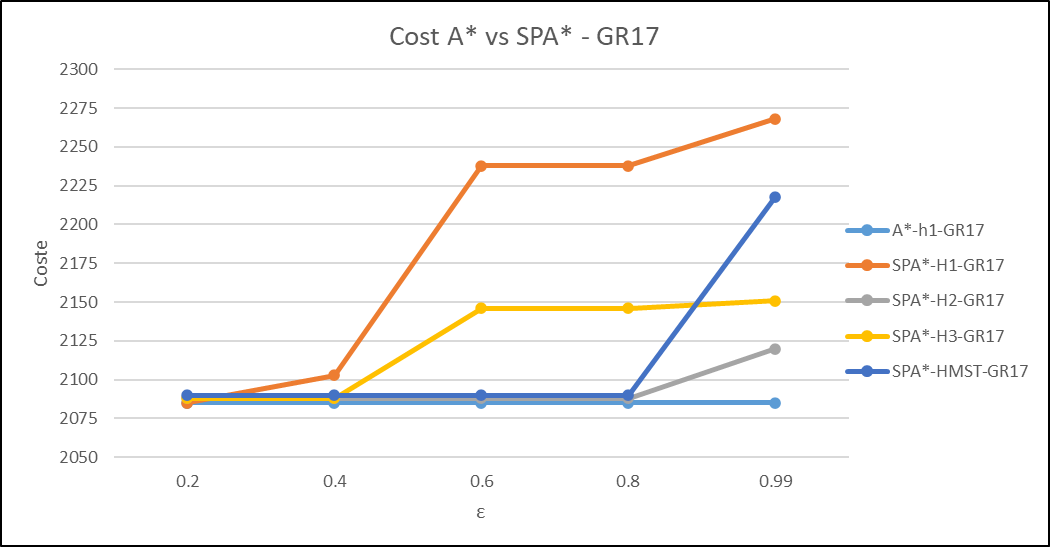
\includegraphics[width=0.7\textwidth]{Graph SPA.png} 
  \caption{Comparison of SPA* Costs with Various $\epsilon$ Values to A* Optimal Cost for the GR17 Instance.}
  \label{fig:alg-cost-comparison}
\end{figure}
\begin{table}[H]
\centering
\caption{SPA* Results for GR17 Instance with Various Heuristics and Epsilons. Time measurements are in seconds.}
\label{tab:spastar-results}
\resizebox{\textwidth}{!}{
\begin{tabular}{|c|c|c|c|c|c|}
\hline
Heuristic & $\epsilon$ & Expanded Nodes & Average (Time) & Standard Deviation (Time) & Length (Cost) \\
\hline
h1 & 0.2 & 30273 & 3.545046353 & 0.223812911 & 2085 \\
 & 0.4 & 11853 & 1.549099922 & 0.17057407 & 2103 \\
 & 0.6 & 4518 & 0.55580008 & 0.167406067 & 2238 \\
 & 0.8 & 1636 & 0.227800226 & 0.128229416 & 2238 \\
 & 0.99 & 478 & 0.077399087 & 0.095782597 & 2268 \\
\hline
h2 & 0.2 & 165565 & 16.91656694 & 1.121160929 & 2088 \\
 & 0.4 & 99602 & 11.38393157 & 1.072885589 & 2088 \\
 & 0.6 & 58289 & 7.193899703 & 0.580293861 & 2088 \\
 & 0.8 & 37246 & 4.845499349 & 0.634438286 & 2088 \\
 & 0.99 & 21205 & 3.06549921 & 0.439285928 & 2120 \\
\hline
h3 & 0.2 & 37236 & 6.12194941 & 0.700358208 & 2088 \\
 & 0.4 & 16477 & 2.947298694 & 0.02590811 & 2088 \\
 & 0.6 & 7335 & 1.345900083 & 0.034099174 & 2146 \\
 & 0.8 & 1643 & 0.345799541 & 0.020394877 & 2146 \\
 & 0.99 & 554 & 0.119900203 & 0.018272382 & 2151 \\
\hline
h\_mst & 0.2 & 11544 & 26.34758334 & 0.114694006 & 2090 \\
 & 0.4 & 4346 & 10.04292498 & 0.051799545 & 2090 \\
 & 0.6 & 1949 & 4.403960323 & 0.038079103 & 2090 \\
 & 0.8 & 1495 & 4.094906282 & 0.033538196 & 2090 \\
 & 0.99 & 730 & 2.903900433 & 0.047827413 & 2218 \\
\hline
\end{tabular}
}
\end{table}
\subsubsection{Algorithm comparison A* vs SPA*}
As evident from Table \ref{tab:astar-results} and Table \ref{tab:spastar-results}, the utilization of SPA* significantly reduces the number of expanded nodes and the time required to obtain a solution, although at the expense of results that deviate further from optimal. The disparity in expanded nodes is visually depicted in Fig. \ref{fig:astar-spastar-comparison}.
\begin{figure}[H]
  \centering
  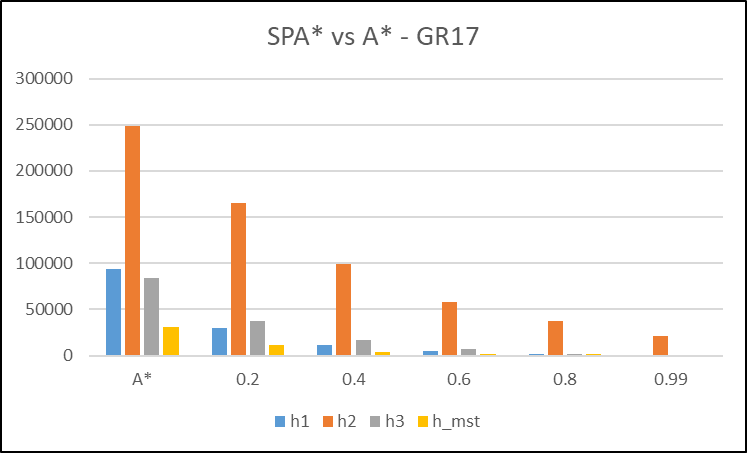
\includegraphics[width=0.7\textwidth]{Graph A vs SPA.png} 
  \caption{Comparison of Expanded Nodes: SPA* with Various $\epsilon$ vs. A* for GR17 Instance Using Four Defined Heuristics.}
  \label{fig:astar-spastar-comparison}
\end{figure}
\subsubsection{Number generations genetic comparison} 
The results indicate that with a higher number of generations, the approach to the optimal cost of the problem improves. However, this improvement is reflected in the time required to achieve it. For instance, with \textit{300} generations, the best cost is closer to the optimum compared to \textit{100} generations, but the time taken is greater with \textit{300}, as illustrated in Tab \ref{tab:ga-results}, Fig. \ref{fig:ox-comparison}, and Fig. \ref{fig:ux-comparison}.

\subsubsection{Crossover Operator comparison OX vs UX}
The results reveal that \textit{OX} is marginally more effective in achieving a solution close to the optimum compared to \textit{UX}. However, the times obtained by both operators across different generations are also relatively comparable. The nuanced difference is apparent in Table \ref{tab:ga-results}, Fig. \ref{fig:ox-comparison}, and Fig. \ref{fig:ux-comparison}.
\begin{table}[H]
\centering
\caption{Genetic Algorithm Results for GR17 with OX and UX Crossover Operators, Varied Number of Generations.}
\label{tab:ga-results}
\resizebox{\textwidth}{!}{
\begin{tabular}{|c|c|c|c|c|c|}
\hline
Crossover Op & N Gens & Best (Avg) & Solution Cost (Avg) & Standard Deviation (Cost) & Average (Time) \\
\hline
OX & 100 & 2497.5 & 2698.686 & 167.8344766 & 1.568090987 \\
   & 150 & 2453.3 & 2681.111333 & 164.0302266 & 2.328969046 \\
   & 200 & 2391.9 & 2552.1625 & 178.4466897 & 3.087874409 \\
   & 250 & 2416.9 & 2572.3112 & 171.8446308 & 3.909895103 \\
   & 300 & 2245.5 & 2448.593 & 245.3503937 & 4.703596943 \\
\hline
UX & 100 & 2548.5 & 2824.911 & 199.4617631 & 1.475074123 \\
   & 150 & 2519.3 & 2732.484667 & 196.5803471 & 2.203592419 \\
   & 200 & 2430.5 & 2631.839 & 218.8820025 & 2.941896438 \\
   & 250 & 2369.7 & 2621.2668 & 228.8854709 & 3.694080231 \\
   & 300 & 2444.5 & 2659.570333 & 201.2008214 & 4.562186526 \\
\hline
\end{tabular}
}
\end{table}

\begin{figure}[H]
  \centering
  \begin{minipage}{0.7\textwidth}
    \centering
    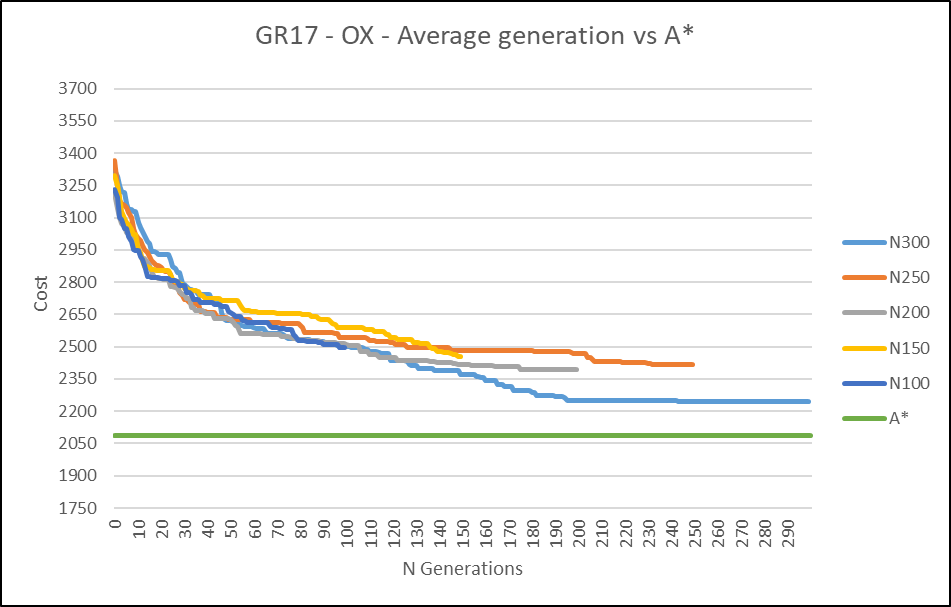
\includegraphics[width=\linewidth]{OX.png}
    \caption{Average Cost Comparison between OX and Different Generations for GR17 Instance, with Four Series Based on Maximum Generation Counts, Alongside the Optimal A* Solution Cost.}
    \label{fig:ox-comparison}
  \end{minipage}
  \hfill
\end{figure}
\begin{figure}[H]
\centering
  \begin{minipage}{0.7\textwidth}
    \centering
    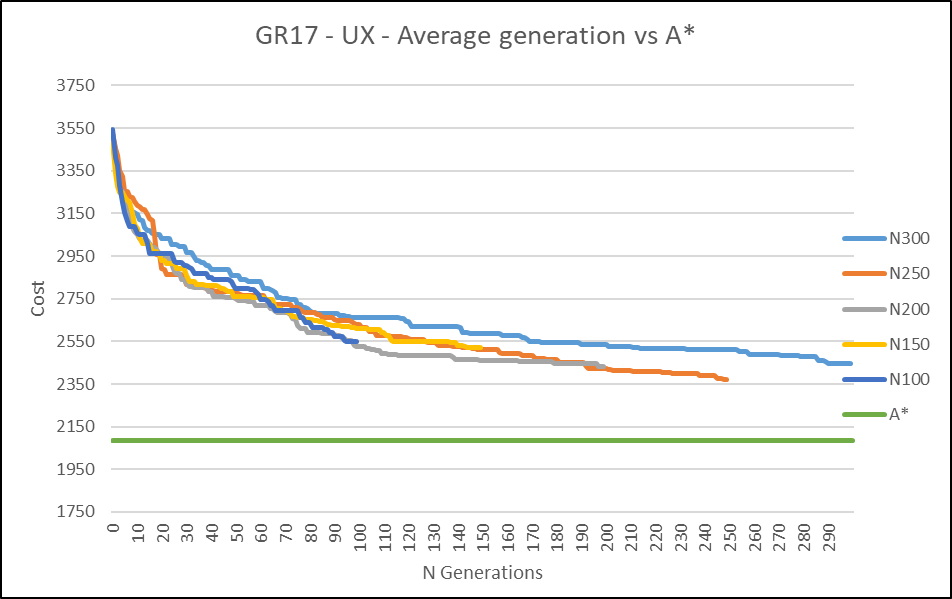
\includegraphics[width=\linewidth]{UX.png}
    \caption{Average Cost Comparison between UX and Different Generations for GR17 Instance, with Four Series Based on Maximum Generation Counts, Alongside the Optimal A* Solution Cost.}
    \label{fig:ux-comparison}
  \end{minipage}
  \hfill
\end{figure}


% 
% Here are the general conclusions of the work. There is no need to repeat the introduction.
%
\section{Conclusions}
As has been demonstrated, the findings presented in this paper lead to the conclusion that employing SPA* allows for the attainment of solutions that may be less precise but in a shorter time compared to A*. A* with the specified heuristics and instances consistently reaches the optimal solution.

Furthermore, the application of genetic algorithms demonstrates the capability to address complex optimization problems. It's noteworthy that achieving a more precise solution is feasible with an increased number of populations and generations in the genetic algorithm approach.

%
% ---- Bibliography ----
%
% BibTeX users should specify bibliography style 'splncs04'.
% References will then be sorted and formatted in the correct style.
%
\bibliographystyle{splncs04}
\bibliography{bibliography}
%

\end{document}
